\section{Functions}

A function is an input/output relationship:~for each
input value there is an output value, and that output value is unique.

One example is the association of each input natural number with 
an output number that is twice as big.
Another is the association of each string of characters over \str{a}--\str{z}
with the length of that string.
A third is the association of each polynomial 
$a_nx^n+\cdots+a_1x+a_0$ with a Boolean value $T$ or~$F$,
depending on whether $1$ is a root of that polynomial.

For the definition fix two sets, 
a \definend{domain}~$D$ and a \definend{codomain}~$C$.
A \definend{function} $\map{f}{D}{C}$ is a set of pairs
$(x,y)\in D\times C$ subject to the restriction that
every element~$x\in D$ appears in one and only one pair.
Where $(x,y)$ is one of the pairs we may write $f(x)=y$ 
or $x\mapsto y$. 
We say that~$x$ is an \definend{input} or \definend{argument} to the function,
and that~$y$ is an \definend{output} or \definend{value}.

The most important point is what a function isn't:~it isn't a 
formula.
The function that gives the presidents of the US, 
$f(0)=\text{George Washington}$, etc., has no sensible formula.
Nor can you produce a formula that returns World Series winners,
including next year's.  
Many functions are described by formulas, such as $f(m)=mc^2$,
and many functions are described by computer programs.
But what makes something a function is not that you can
compute it, instead it is that for each input 
from the domain there is one and only one output from the codomain.

\subsection{Pictures}
We may illustrate functions using the familiar $xy$~axes;
here are the graphs of $f(x)=x^3$ and $f(x)=\floor{x}$.
\begin{center}
  \vcenteredhbox{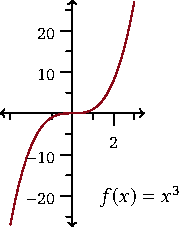
\includegraphics{appendix/asy/functions000.pdf}}
  \hspace{2em plus 0.5fil}
  \vcenteredhbox{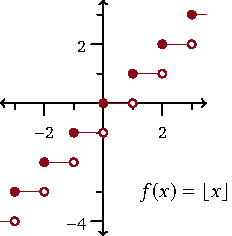
\includegraphics{appendix/asy/functions001.pdf}}
\end{center}
We also sometimes depict functions using a bean diagram, 
which separates the domain from the codomain.
On the left below it pictures the action of the exclusive~or operator. 
\begin{center}
  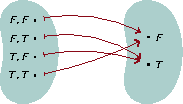
\includegraphics{appendix/asy/functions002.pdf}
  \hspace{2em plus 1fil}
  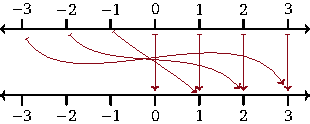
\includegraphics{appendix/asy/functions005.pdf}
\end{center}
On the right is a variant of the bean diagram, showing the
absolute value function mapping the integers to the integers.

\subsection{Codomain and range}
Where  $S\subseteq D$ is a subset of the domain, its \definend{image} 
is $f(S)=\set{f(s)\suchthat s\in S}$.
Thus, under the floor function the image of the positive reals is
the nonnegative reals.
The image of the entire domain is the \definend{range}
of the function, $f(D)=\operatorname{ran}(f)$.
Note that the range is not the same as the codomain;
instead, the codomain is a convenient superset.
For instance, for the real function $f(x)=x^2$ we may write $\map{f}{\R}{\R}$,
although the range is the nonnegative reals. 

When we are defining a function and write 
$\map{f}{D}{C}$ we need that
every $f(x)$ is indeed an element of~$C$; usually it is clear but 
on occasion we need to say a bit more.

\subsection{Domain}
The flip side is that sometimes the domain is not OK.
Examples from Calculus of troublesome real number functions
are that $f(x)=1/x$ 
is undefined at $x=0$, or that the infinite series
$f(r)=1+r+r^2+\cdots$ diverges when $r$ is outside the interval
$\open{-1}{1}$.
Formally, we must specify the function's domain so that no such problem happens.
Restriction of a function.  

However, we are often casual about this and in this subject
if there are some elements of the domain where the function
is undefined we will say that it is a \definend{partial function} (otherwise
it is a \definend{total function}).

\subsection{Well-defined}
The definition of a function has  
the restriction that for 
every domain element there is one and only one associated
codomain element~$y=f(x)$.
Because of this we say functions are \definend{well-defined}.

We sometimes consider a relationship between some $x$'s and $y$'s and
ask ourselves if it satisfies the restriction.
For instance, in Calculus we sometimes have to deal with the fact that
positive real numbers have more than one square root.
Or, if we are setting up a company's email we may decide to use a person's
first initial and last name but then realize that
there can easily be more than one, say, \str{rjones}.
We say that the mapping from address to person is not well-defined, 
or `ill-defined'.\footnote{%
  Sometimes people say that they are, ``checking that the function is 
  well-defined.''
  In a strict sense that sentence is confused, or at least awkward, since   
  if it is a function then it is by definition well-defined.
  However, all tigers have stripes but we do
  sometimes say ``striped tiger;''; natural language is funny that way.
  }



\subsection{One-to-one and onto}
Asymmetry in restriction between domain and codomain.

Defn, showing one-to-one.
\begin{center}
  \vcenteredhbox{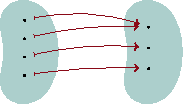
\includegraphics{appendix/asy/functions003.pdf}}
\end{center}
Graphically checking  one-to-one on xy plot with horizontal line.

For finite sets.

Defn, showing onto.
\begin{center}
  \vcenteredhbox{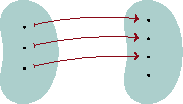
\includegraphics{appendix/asy/functions004.pdf}}
\end{center}
Graphically checking onto on xy plot with horizontal line.

For finite sets.

\subsection{Correspondence}
Defn, showing correspondence.
Graphical correspondence on xy plot with horizontal line.

Correspondence for finite sets.